
\chapter{Overview about vector fields and segmentation techniques}
\section{The vector field}
What is a vector field? A Vector field is an assignment of a vector to each point in a subset of space. This assignment is the value that will give an orientation to the row that will describe our image.
\begin{figure}
	\centering
	\begin{subfigure}[b]{0.5\textwidth}
        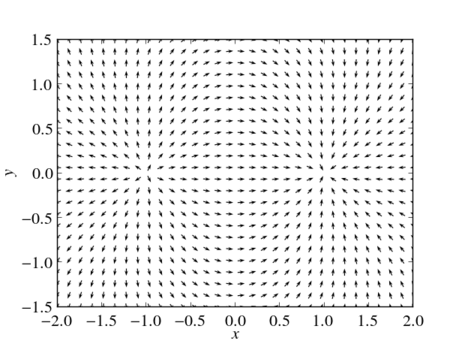
\includegraphics[width=\textwidth]{img/fieldex.png}
        \caption{ }
        \label{fig:field}
    \end{subfigure}
    \begin{subfigure}[b]{0.5\textwidth}
		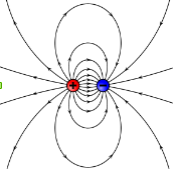
\includegraphics[width=\textwidth]{img/dipole.png}
		\caption{ }
		\label{fig:dipole}
	\end{subfigure}
	\caption{(a) Dipole electric field, (b) Electric dipole}
	\label{fig:fielddipole}
\end{figure}
The figure \ref{fig:fielddipole} represent a vector field flow of an electric dipole \ref{fig:dipole} in the $x-y-plane$ with $r+=(-1,0,0) and r-=(1,0,0)$. All vectors are normalized to the unity. Thus, the plot visualizes the direction of the electric dipole field, but not the field strength. In the negative zone part of the dipole it is possible to see that rows of the vector field tries to enter the plane and at the opposite side it’s possible to see the exact opposite, that shows the rows exit from the plane. This translates into a flow of rows that is possible to applicate to describe the leukocyte's edges.

Active contours, also called snakes, are curves that move inside the image following the energy of the field. There are two kinds of forces, one internal and anther external. Combining these two it's possible to create a curve that follows constraints gives by the forces. The  internal  and  external  forces  are  defined  so  that  the  snake  will conform to an object boundary or other desired features within an image. Snakes are widely used  in  many  applications,  including  edge  detection,  shape  modelling and segmentation. There  are  two  general  types  of  active  contour  models  in  the literature  today:  parametric active contours and geometric active contours. Typically,  the  curves  are  drawn  toward  the edges  by  potential  forces,  which  are  defined  to  be  the  negative  gradient  of  a  potential function.  Additional  forces,  such  as  pressure  forces,  together  with  the  potential  forces comprise the external forces. There are also internal forces designed to hold the curve together and to keep it from bending too  much.  There  are  two  levels  difficulties  with  active  contour  algorithms.  First,  the  initial contour must be close to the true boundary or else it will likely converge to the wrong result. The second problem is that active contours have difficulties progressing into concave  boundary  regions.  Although  many  methods  such  as  multi resolution  methods, pressure forces, distance potential forces, control points, and using solenoidal external fields have been proposed they either solve one problem or solve both but creating new difficulties. For  example,  multi resolution  methods  have  addressed  the  issue  of  initialization,  but specifying  how  the  snake  should  move  across  different  resolutions  remains  problematic. Another example is that of pressure forces, which can push an active contour into boundary concavities, but cannot be too strong or “weak” edges will be overwhelmed. But how works a snake if the objects to segment are overlapped? Snakes are able to find all the external edges of the object but in this case the edge can be consider an internal part of the object. With the active contours is impossible segment the overlapped cells because the snake cannot enter inside the cell region. For these reason we have used our virtual field following another lecture key.

\section{An overview of Image Segmentation methods}
when we talking about segmentation we introduce a technique for partitioning the image into subregions. Below are described the most five famous techniques to develop an image segmentation:
\begin{enumerate}
	\item threshold-based;
	\item histogram-based;
	\item region-based;
	\item edge detection;
	\item watershed transformation
\end{enumerate}
\subsection{threshold-based techniques}
Thresholding is the simplest segmentation method. The pixels are partitioned depending on their intensity value generally used with gray scale images $f(x,y)$. When the threshold is apply on gray scale images the final target is separate the foreground by the background. The first one contains only the element of interest and the second one contains all the rest of the image. The global threshold value T is the 'breaking point' of the image. After an analysis of the image, the value T is used to understand if, taking in account each pixel of the image,each one it belongs to the foreground $f(x, y) > T$ or to the background $f(x, y) < T$ . used to understand if, taking in analysis each pixel of the image, it's below to the foreground $f(x, y) > T$ or to the background$f(x, y) < T$.\cite{Threshold}

\subsection{Histogram-based techniques}
An important class of point operations is based upon the manipulation of an image histogram or a region histogram